\documentclass[tikz, border = 2pt]{standalone}

%---------------------------------------------------------------------------%
% PACKAGES                                                                  %
%---------------------------------------------------------------------------%

%----- MATH
%---------------------------------------------------------------------------%
\usepackage{amsmath, amssymb}

%----- FIGURES
%---------------------------------------------------------------------------%
\usepackage{pgfplots}
\pgfplotsset{compat=1.13}


\begin{document}

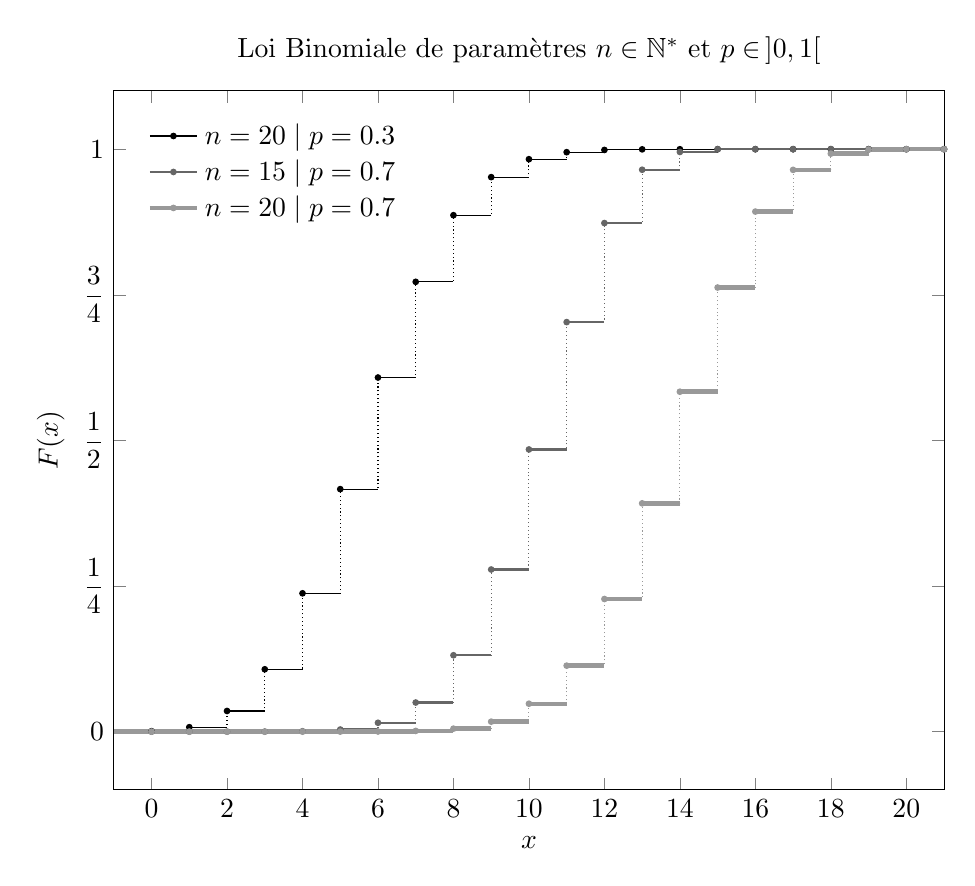
\begin{tikzpicture}
\begin{axis}[width = \textwidth,
title style = {align = center},
title={Loi Binomiale de param\`etres $n \in \mathbb{N}^\ast$ et $p \in\, ]0,1[$},
xlabel={$x$},
ylabel={$F(x)$},
legend pos = north west,
legend style = {draw=none},
xmin = -1,
xmax = 21,
ytick = {0,0.25,0.5,0.75,1},
yticklabels = {$0$, $\dfrac{1}{4}$, $\dfrac{1}{2}$, $\dfrac{3}{4}$, $1$},
ylabel near ticks
]
\addplot[mark = none, black, thin, const plot, densely dotted, forget plot] coordinates {(-1,0) (0,0.000797922662976119) (1,0.0076372597742) (2,0.0354831322984687) (3,0.107086804503731) (4,0.237507778877601) (5,0.416370829447481) (6,0.608009812200924) (7,0.772271797418161) (8,0.886668537123022) (9,0.952038102668657) (10,0.982855183568742) (11,0.994861838464879) (12,0.99872112039578) (13,0.999738952992941) (14,0.999957059978046) (15,0.999994449746922) (16,0.999999457305253) (17,0.999999962269119) (18,0.999999998337966) (19,0.999999999965132) (20,1) (21,1)};
\addplot[mark = none, black, forget plot, domain = -1:0] {0};
\addplot[black, jump mark left, mark=*, mark size = 1pt, mark options = {thin, fill = black}] coordinates {(0,0.000797922662976119) (1,0.0076372597742) (2,0.0354831322984687) (3,0.107086804503731) (4,0.237507778877601) (5,0.416370829447481) (6,0.608009812200924) (7,0.772271797418161) (8,0.886668537123022) (9,0.952038102668657) (10,0.982855183568742) (11,0.994861838464879) (12,0.99872112039578) (13,0.999738952992941) (14,0.999957059978046) (15,0.999994449746922) (16,0.999999457305253) (17,0.999999962269119) (18,0.999999998337966) (19,0.999999999965132) (20,1) (21,1)};
%
\addplot[mark = none, black!60, thin, const plot, densely dotted, forget plot] coordinates {(-1,0) (0,1.4348907e-08) (1,5.16560652e-07) (2,8.71935248700001e-06) (3,9.16586921520001e-05) (4,0.000672234069807001) (5,0.00365252100843601) (6,0.015242525769771) (7,0.0500125400537761) (8,0.131142573383121) (9,0.278378559795636) (10,0.484508940773157) (11,0.703132072112952) (12,0.873172285377237) (13,0.964732400211852) (14,0.995252438490057) (15,1) (16,1) (17,1) (18,1) (19,1) (20,1) (21,1)};
\addplot[mark = none, black!60, thick, forget plot, domain = -1:0] {0};
\addplot[black!60, thick, jump mark left, mark=*, mark size = 1pt, mark options = {thin, fill = black!60}] coordinates {(0,1.4348907e-08) (1,5.16560652e-07) (2,8.71935248700001e-06) (3,9.16586921520001e-05) (4,0.000672234069807001) (5,0.00365252100843601) (6,0.015242525769771) (7,0.0500125400537761) (8,0.131142573383121) (9,0.278378559795636) (10,0.484508940773157) (11,0.703132072112952) (12,0.873172285377237) (13,0.964732400211852) (14,0.995252438490057) (15,1) (16,1) (17,1) (18,1) (19,1) (20,1) (21,1)};

\addplot[mark = none, black!40, thin, const plot, densely dotted, forget plot] coordinates {(-1,0) (0,3.486784401e-11) (1,1.66203389781e-09) (2,3.77308814237101e-08) (3,5.42694746786311e-07) (4,5.55025307829877e-06) (5,4.29400219535918e-05) (6,0.000261047007059468) (7,0.00127887960422022) (8,0.00513816153512141) (9,0.0171448164312585) (10,0.0479618973313436) (11,0.113331462876979) (12,0.22772820258184) (13,0.391990187799077) (14,0.583629170552519) (15,0.762492221122398) (16,0.892913195496269) (17,0.964516867701531) (18,0.9923627402258) (19,0.999202077337024) (20,1) (21,1)};
\addplot[mark = none, black!40, ultra thick, forget plot, domain = -1:0] {0};
\addplot[black!40, ultra thick, jump mark left, mark=*, mark size = 1pt, mark options = {thin, fill = black!40}] coordinates {(0,3.486784401e-11) (1,1.66203389781e-09) (2,3.77308814237101e-08) (3,5.42694746786311e-07) (4,5.55025307829877e-06) (5,4.29400219535918e-05) (6,0.000261047007059468) (7,0.00127887960422022) (8,0.00513816153512141) (9,0.0171448164312585) (10,0.0479618973313436) (11,0.113331462876979) (12,0.22772820258184) (13,0.391990187799077) (14,0.583629170552519) (15,0.762492221122398) (16,0.892913195496269) (17,0.964516867701531) (18,0.9923627402258) (19,0.999202077337024) (20,1) (21,1)};

\legend{{$n=20 \mid p = 0.3$}, {$n=15 \mid p=0.7$}, {$n=20 \mid p = 0.7$}}
\end{axis}
\end{tikzpicture}

\end{document}